\documentclass[11pt]{article}
%prepared in AMSLaTeX, under LaTeX2e
\addtolength{\oddsidemargin}{-.75in} 
\addtolength{\evensidemargin}{-.75in}
\addtolength{\topmargin}{-.6in}
\addtolength{\textwidth}{1.4in}
\addtolength{\textheight}{1.3in}

\renewcommand{\baselinestretch}{1.06}

\usepackage{wrapfig,fancyvrb,xspace}
\usepackage{palatino,amsmath,amssymb,amsthm}
\usepackage[final]{graphicx}
\usepackage[pdftex, colorlinks=true, plainpages=false, linkcolor=blue, citecolor=red, urlcolor=blue]{hyperref}

% macros
\newcommand{\RR}{\mathbb{R}}
\newcommand{\grad}{\nabla}
\newcommand{\lam}{\lambda}
\newcommand{\ds}{\displaystyle}
\newcommand{\Matlab}{\textsc{Matlab}\xspace}


\title{POPDIP: a POsitive-variables \\ Primal-Dual Interior Point optimization method}
\author{Ed Bueler}
\date{Version 1.2.  4 November 2024}

\begin{document}
\maketitle

\begin{abstract}
The algorithm here is an example of the Newton-type primal-dual interior point algorithms presented in \cite[section 16.7]{GrivaNashSofer2009}, \cite[chapter 19]{NocedalWright2006}, and \cite{YamashitaYabe1996}.  It minimizes a smooth nonlinear function subject to the constraints that all the variables are nonnegative, plus linear equality constraints:
\begin{equation}
\begin{matrix}
\text{minimize} \qquad   & f(x) \\
\text{subject to} \qquad & A x = b \\
                         & x \ge 0
\end{matrix} \label{eq:problem}
\end{equation}
The algorithm here is specialized for nonnegativity constraints $x\ge 0$, and it is not suitable for general inequality constraints of the form ``$g_i(x)\ge 0$.''  Nor is it suitable for general equality constraints ``$g_i(x)=0$.''  However, it can be used as an interior-point method for linear programming (LP), that is, in the case where $f(x)=c^\top x$.  This method can therefore solve LP problems in standard form, but it has no special performance improvements for that case.

These short notes are \emph{not} research.  I simply implement a special case of a well-known algorithm.  Furthermore ``POPDIP'' is a name I made up; it is not in common use.  I have implemented this case because I am interested in interior point methods.

Download the code, this documentation, slides, and the examples by cloning the Github repository \href{https://github.com/bueler/popdip}{\texttt{github.com/bueler/popdip}},
or get an archive from the same site.\end{abstract}

\thispagestyle{empty}

\bigskip
\subsection*{Introduction}

First consider a nonlinear optimization problem with only nonnegativity (informally: positivity) constraints on the variables:
\begin{equation}
\begin{matrix}
\text{minimize} \qquad & f(x) \\
\text{subject to} \qquad & x \ge 0
\end{matrix} \label{eq:posproblem}
\end{equation}
As usual, $x\ge 0$ in \eqref{eq:posproblem} means that each entry of $x\in\RR^n$ is nonnegative.  The feasible set for \eqref{eq:posproblem} is the convex and closed set $S = \{x\in \RR^n\,:\,x\ge 0\}$, with interior $S^\circ = \{x\in \RR^n\,:\,x > 0\}$, and $f:S \to \RR$ is assumed to be a continuous and smooth function.  (The next section will address the general problem \eqref{eq:problem} including linear equality constraints.)

One can derive an interior point method for \eqref{eq:posproblem} by considering a logarithmic barrier function \cite[section 16.2]{GrivaNashSofer2009}.  Let $\mu>0$ be a (temporarily) fixed constant.  If $x\in S^\circ$ then the following function is well-defined:
\begin{equation}
\beta_\mu(x) = f(x) - \mu \sum_{i=1}^n \ln x_i \label{eq:posbarrierfunction}
\end{equation}
Recalling that $\lim_{x\to 0^+} \ln x = -\infty$, this barrier imposes ``infinite cost'' to reaching the boundary of the feasible set $S$.

Now let $\{e_1,\dots,e_n\}$ be the standard basis of $\RR^n$.  The first-order necessary condition for the \emph{unconstrained} problem of minimizing $\beta_\mu$, namely $\grad \beta_\mu(x)=0$ for $x \in S^\circ$, is
\begin{equation}
\grad f(x) - \mu \sum_{i=1}^n \frac{1}{x_i} e_i = 0 \label{eq:posfirstorderbarrier}
\end{equation}

Conditions \eqref{eq:posfirstorderbarrier} can be reformulated by defining additional variables
\begin{equation}
\lambda_i = \frac{\mu}{x_i} \label{eq:poslocktogether}
\end{equation}
so that $\lambda\in\RR^n$.  Note that $\lambda>0$ if and only if $x>0$ because $\lambda_i x_i = \mu > 0$.  Equations \eqref{eq:posfirstorderbarrier} and \eqref{eq:poslocktogether}, plus feasibility for $x$, form the following nonlinear system of equations and inequalities:
\begin{align}
\grad f(x) - \lambda &= 0 \label{eq:posfirstordersystem} \\
\lambda_i x_i &= \mu, \qquad i=1,\dots,n \notag \\
x &\ge 0 \notag \\
\lambda &\ge 0 \notag
\end{align}
Because of the second condition in system \eqref{eq:posfirstordersystem}, both $x$ and $\lambda$ are strictly positive and thus in the interior $S^\circ$.

The first condition in system \eqref{eq:posfirstordersystem} can be rewritten as $\grad_x \mathcal{L}(x,\lambda)=0$ using this Lagrangian function for problem \eqref{eq:posproblem}:
\begin{equation}
\mathcal{L}(x,\lambda) = f(x) - \sum_{i=1}^n \lambda_i x_i.  \label{eq:poslagrangian}
\end{equation}
The first-order KKT conditions \cite[sections 14.4, 14.5]{GrivaNashSofer2009} of problem \eqref{eq:posproblem}, which one can derive using Lagrangian \eqref{eq:poslagrangian}, are nearly the same as the condition in \eqref{eq:posfirstordersystem} but with the second equation replaced by complementarity,
\begin{align}
\grad f(x) - \lambda &= 0 \label{eq:poskkt} \\
\lambda_i x_i &= 0, \qquad i=1,\dots,n \notag \\
x &\ge 0 \notag \\
\lambda &\ge 0 \notag
\end{align}

Now we see that, though a logarithmic barrier method generated system \eqref{eq:posfirstordersystem}, the system can also be derived by a modification of KKT conditions \eqref{eq:poskkt}.  The modification changes the complementarity condition into a nonzero connection between the primal and dual variables.  (Their product is set to a positive constant.)  System \eqref{eq:posfirstordersystem} describes a primal and dual $(x,\lambda)$ solution which is interior to the feasible set, and thus different from the solution to \eqref{eq:poskkt}, but the former approximates the latter if $\mu>0$ is small.

The first condition in \eqref{eq:poskkt} allows $\lambda$ to be eliminated if desired: $\lambda = \grad f(x)$.  Writing the KKT conditions \eqref{eq:poskkt} without these dual variables gives a \emph{nonlinear complementarity problem} (NCP) \cite{FacchineiPang2007},
\begin{equation}
x \ge 0, \qquad \grad f(x) \ge 0, \qquad x_i (\grad f(x))_i = 0.  \label{eq:posncp}
\end{equation}
Thus we may regard POPDIP as solving the $\mu$-modified NCP
\begin{equation}
x \ge 0, \qquad \grad f(x) \ge 0, \qquad x_i (\grad f(x))_i = \mu. \label{eq:mumodifiedncp}
\end{equation}
However, POPDIP can achieve quadratic convergence substantially because it updates primal and dual variables separately.  Stating the algorithm or the original KKT conditions as an NCP, thereby suppressing the dual variables, is not beneficial to solver performance.  On the other hand, such NCP formulations also appear in problems which are not optimizations, rather variational inequalities, and I am focussed these days on glaciological variational inequalities \cite{Bueler2016,BuelerFarrell2024}, for example.


\subsection*{General problem}

Suppose from now on that $f:\RR^n \to \RR$ is twice continuously-differentiable.  Let $A\in\RR^{m\times n}$, $m\le n$, be a full rank matrix, and suppose $b\in\RR^m$.  The POPDIP algorithm solves general problems of form \eqref{eq:problem} given in the abstract and restated here:
\begin{equation}
\begin{matrix}
\text{minimize} \qquad   & f(x) \\
\text{subject to} \qquad & A x = b \\
                         & x \ge 0
\end{matrix} \tag{1}
\end{equation}

Observe that the constraints are in standard form for linear programming (LP) problems \cite[chapter 4]{GrivaNashSofer2009}.  If $f(x)=c^\top x$ for some fixed $c\in\RR^n$ then \eqref{eq:problem} is an LP problem in standard form, and then POPDIP becomes an LP interior point method, though one with no special adaptations to that case; compare e.g.~\cite{ZhangTapiaDennis1992}.

The (primal) feasible set is
\begin{equation}
S = \{Ax=b \text{ and } x\ge 0\} \subset \RR^n.  \label{eq:primalfeasible}
\end{equation}
The iterates $x_k$ from our algorithm will be in the interior,\footnote{In general, $S^o$ is not the topological interior of $S \subset \RR^n$, which is empty when equality constraints apply ($m>0$).} defined to be
\begin{equation}
S^o = \{Ax=b \text{ and } x > 0\} \subset \RR^n.  \label{eq:primalinterior}
\end{equation}
We will assume that $S^o$ is nonempty and that a feasible iterate in $S^o$ can be found.  (In fact the user will \emph{not} need to provide an initial iterate which is feasible with respect to ``$Ax=b$'', but they will need to provide a strictly-positive initial iterate.)

Consider the following Lagrangian for \eqref{eq:problem}:
\begin{equation}
\mathcal{L}(x,\tau,\lambda) = f(x) - \tau^\top (Ax - b) - \lambda^\top x, \label{eq:lagrangian}
\end{equation}
for multipliers $\tau\in\RR^m$ and $\lambda\in \RR^n$.  Notice that \eqref{eq:lagrangian} reduces to \eqref{eq:poslagrangian} if there are $m=0$ linear equality constraints (and thus $\tau$ is absent).

The first-order necessary conditions, the KKT conditions, for \eqref{eq:problem} are given by $\grad_x\mathcal{L}=0$ and $\grad_\tau\mathcal{L}=0$, plus complementarity for the primal variables $x$ and dual variables $\lambda$:
\begin{align}
\grad f(x) - A^\top \tau - \lambda &= 0 \label{eq:kkt} \\
-A x + b &= 0 \notag \\
\lambda_i x_i &=0, \qquad i=1,\dots,n \notag \\
x &\ge 0 \notag \\
\lambda &\ge 0 \notag
\end{align}
Conditions \eqref{eq:kkt} reduce to system \eqref{eq:poskkt} given in the Introduction when there are $m=0$ linear equality constraints.  Note that the dual feasible set $\{\lambda \ge 0\}\subset \RR^n$ is generally different from, and larger than, the primal feasible set $S$.


\subsection*{Algorithm design}

The POPDIP algorithm solves \eqref{eq:problem} by applying a Newton method to a $\mu$-modified form of KKT conditions \eqref{eq:kkt}.  The modification replaces complementarity $\lambda_i x_i = 0$ by the conditions
\begin{equation}
\lambda_i x_i = \mu_k, \qquad i=1,\dots,n \notag \\
\end{equation}
for a (scalar) barrier sequence $\mu_k>0$ which will go to zero.  Thus POPDIP computes primal and dual iterates in the interiors: $x \in S^o$, $\lambda > 0$.  However, if the method converges as $\mu_k \to 0$ then the limiting values of $x$ and $\lambda$ solve the KKT conditions \eqref{eq:kkt}.  Though the algorithm is terminated after a finite number of steps, we will see in examples that the KKT system can be solved to high accuracy.

Each step of the algorithm is a Newton step for the modified equalities from \eqref{eq:kkt}, namely
\begin{align}
\grad f(x) - A^\top \tau - \lambda &= 0 \label{eq:equalities} \\
-A x + b &= 0 \notag \\
\lambda_i x_i &= \mu_k, \qquad i=1,\dots,n \notag
\end{align}
Because of its third equation, \eqref{eq:equalities} is always a nonlinear system.  However, if $f$ is quadratic or linear then \emph{only} the third equation, the modified complementarity condition, is nonlinear.

Intuitively, an interior-point iteration for \eqref{eq:equalities} solves ``changing equations'' with iteration $k$.  As we update the $\mu_k$ value, each new iterate is attempting to solve new equations.  Thus, though the iterates of POPDIP should converge to the solution of KKT problem \eqref{eq:kkt}, they will not converge to a solution of \eqref{eq:equalities} for any particular $\mu_k>0$.

The Newton step computes a search direction in the $x,\tau,\lambda$ variables using the linearization of equations \eqref{eq:equalities}, but POPDIP uses different step sizes for the three variables.  A ratio test \cite[section 3.1]{GrivaNashSofer2009} restricts the step sizes for $x$ and $\lambda$, the variables subject to inequality constraints.

To describe the Newton step in detail, let $x=x_k+\Delta x$, $\tau=\tau_k+\Delta\tau$ and $\lambda=\lambda_k+\Delta\lambda$.  The unknowns form a candidate search direction $p=(\Delta x,\Delta\tau,\Delta\lambda)$; it will be modified later.  Substituting into \eqref{eq:equalities} and expanding to first order gives
\begin{align}
\grad f(x_k) + \grad^2 f(x_k) \Delta x - A^\top \tau_k - A^\top \Delta \tau - \lambda_k - \Delta \lambda &= 0 \label{eq:prenewtonstep} \\
-A x_k - A \Delta x + b &= 0 \notag \\
(\lambda_k)_i (x_k)_i + (x_k)_i (\Delta\lambda)_i + (\lambda_k)_i (\Delta x)_i &= \mu_k, \qquad i=1,\dots,n \notag
\end{align}
Rearranging this as a matrix-block system gives
\begin{equation}
\begin{bmatrix}
\grad^2 f(x_k) & -A^\top & -I \\
-A             & 0       & 0  \\
\Lambda_k      & 0       & X_k
\end{bmatrix}
\begin{bmatrix}
\Delta x \\
\Delta \tau \\
\Delta \lambda
\end{bmatrix}
=
\begin{bmatrix}
-\grad f(x_k) + A^\top \tau_k + \lambda_k \\
A x_k - b \\
\mu_k e - \Lambda_k x_k
\end{bmatrix}. \label{eq:unreducednewtonstep}
\end{equation}
Here $I$ is the $n\times n$ identity matrix, $e=(1,1,\dots,1)^\top \in \RR^n$, and we have defined $n\times n$ diagonal matrices from the primal/dual vectors $x,\lambda\in\RR^n$ as follows:
    $$X = \begin{bmatrix} x_1 & & \\ & \ddots & \\ & & x_n \end{bmatrix}, \qquad \Lambda = \begin{bmatrix} \lambda_1 & & \\ & \ddots & \\ & & \lambda_n \end{bmatrix}.$$
Note that $\Lambda x = X \lambda$ in this notation.\footnote{The product $\Lambda x = X\lambda$ is simply \, \texttt{x.*lambda}\, in \Matlab.}

For a given $\mu_k>0$ we may consider the \emph{residual function} of system \eqref{eq:equalities}:
\begin{equation}
r_k(x,\tau,\lambda) = \begin{bmatrix}
\grad f(x) - A^\top \tau - \lambda \\
- A x + b \\
\Lambda x - \mu_k e
\end{bmatrix}. \label{eq:residualnewtonstep}
\end{equation}
Using this notation, linear system \eqref{eq:unreducednewtonstep} can be written as
\begin{equation}
M_k p = - r_k \label{eq:overallnewtonstep}
\end{equation}
where $M_k$ is the $(2n+m) \times (2n+m)$ square and sparse \emph{system matrix} on the left side of \eqref{eq:unreducednewtonstep} and $r_k=r_k(x_k,\tau_k,\lambda_k) \in \RR^{2n+m}$ is the residual for the current iterate.

However, system \eqref{eq:unreducednewtonstep} can be made smaller by noting that the diagonal matrix $X_k$ is invertible, because $x_k>0$ strictly in \eqref{eq:equalities}.  Thus the last row of system \eqref{eq:unreducednewtonstep} can be solved for $\Delta\lambda$ in terms of $\Delta x$:
\begin{equation}
\Lambda_k\Delta x + X_k\Delta \lambda = \mu_k e - \Lambda_k x_k \quad \iff \quad
\Delta\lambda = \mu_k X_k^{-1} e - \lambda_k - X_k^{-1} \Lambda_k \Delta x \label{eq:solvefordlam}
\end{equation}
In fact, instead of \eqref{eq:unreducednewtonstep} we will actually solve the smaller, \emph{symmetric} system
\begin{equation}
\begin{bmatrix}
\grad^2 f(x_k) + X_k^{-1}\Lambda_k & -A^\top \\
-A             & 0
\end{bmatrix}
\begin{bmatrix}
\Delta x \\
\Delta \tau
\end{bmatrix}
=
\begin{bmatrix}
-\grad f(x_k) + A^\top \tau_k + \mu_k X_k^{-1} e \\
A x_k - b
\end{bmatrix} \label{eq:newtonstep}
\end{equation}
for $\Delta x,\Delta\tau$, and then complete the Newton step computation by assigning
\begin{equation}
\Delta\lambda = \mu_k X_k^{-1} e - \lambda_k - X_k^{-1} \Lambda_k \Delta x. \label{eq:newtonsteplam}
\end{equation}
The Appendix gives a proof that the block matrix in \eqref{eq:newtonstep} is invertible if the Hessian $\grad^2 f(x_k)$ is positive semi-definite.

We will solve system \eqref{eq:newtonstep} using direct linear algebra, via Matlab's default ``$\backslash$'' linear solver.  Because this direct solver is quite accurate, the residual norm $\|b-A x_k\|$, part of the right-hand side of \eqref{eq:newtonstep}, will be very small.  In this sense, system \eqref{eq:newtonstep} imposes the classical null-space requirement on the (primal) search direction for linear equality constraints \cite[chapter 3]{GrivaNashSofer2009}:
\begin{equation}
A \Delta x = 0.  \label{eq:dxnull}
\end{equation}
Note there is no equivalent linear restriction on $\Delta\lambda$; the direction of $\Delta\lambda$ is unrestricted.

On the other hand, use of a direct solver means the implementation is not scalable to large problem sizes.  A scalable implementation would not assemble the full matrix in \eqref{eq:newtonstep}, and it might use an iterative solver, along the way exploiting the block structure.  Preconditioners \cite{Bueler2021,TrefethenBau1997} for the upper-left block, and then for the Schur complement \cite[chapter 14]{Bueler2021} as well, should be considered.

Given a solution $(\Delta x,\Delta\tau,\Delta\lambda)$ of \eqref{eq:newtonstep} and \eqref{eq:newtonsteplam}, the update formulas are
\begin{align}
x_{k+1} &= x_k + \alpha_x \Delta x \label{eq:updates} \\
\tau_{k+1} &= \tau_k + \alpha_\tau \Delta \tau \notag \\
\lambda_{k+1} &= \lambda_k + \alpha_\lambda \Delta \lambda \notag
\end{align}
Separate step sizes $\alpha_x,\alpha_\tau,\alpha_\lambda$ are used for the three vector variables $x,\tau,\lambda$.  (There are other strategies in the literature, e.g.~\cite{YamashitaYabe1996}.)  In fact, because the constraint equations in \eqref{eq:problem} are linear, the full Newton step $\alpha_\tau=1$ is always used for the $\tau$ multipliers.

Quadratic convergence of a general primal-dual interior point method is proven in subsection 16.7.2 of \cite{GrivaNashSofer2009}.  That method replaces general inequality constraints $g_i(x)\ge 0$ by $g_i(x) - s_i =0$, with slack variables $s_i\ge 0$.  However, in our case this replacement says $x_i-s_i=0$ and $s_i\ge 0$, clearly unneeded as it simply renames existing primal variables $x$.  Also, the back-tracking globalization of the inequality constraints described in algorithm 16.1 of \cite{GrivaNashSofer2009}, which chooses $\alpha_x$ from $\{1,1/2,1/4,\dots\}$ so that $g_i(x_k + \alpha_x \Delta x) > 0$, is not needed to maintain primal feasibility because of the linearity of the constraint functions in \eqref{eq:problem}.  That is, for constraints $Ax=b$ and $x\ge 0$ a ratio test for $\Delta x$ will guarantee primal feasibility, as in the simplex method \cite[chapter 5]{GrivaNashSofer2009}.

POPDIP will shorten the step in the Newton search direction \emph{only} because of the inequality constraints, and not for the ``usual'' (unconstrained) line search reasons, for instance to generate sufficient decrease of $f$ by an Armijo or Wolfe rule \cite[section 11.5]{GrivaNashSofer2009}.  In this sense our method is most suitable for quadratic functions $f$, and it may need additional refinements for more general, especially non-convex, objective functions.  For example, it should be used with caution if the Hessian $\grad^2 f(x)$ varies significantly during the iteration.

POPDIP determines step sizes $\alpha_x,\alpha_\lambda$ for the inequality-constrained primal and dual variables via a condition of (strict) positivity for $x_{k+1}$ and $\lambda_{k+1}$.  Suppose $0<\kappa<1$.  For the primal variables, assuming $x_k\in S^o$ so that $x_k>0$, we require that for all $i$ such that $(\Delta x)_i < 0$,
\begin{equation}
(x_k)_i + \alpha_x (\Delta x)_i \ge (1-\kappa) (x_k)_i \qquad \iff \qquad \alpha_x \le - \kappa \frac{(x_k)_i}{(\Delta x)_i}. \label{eq:preratio}
\end{equation}
(If $(\Delta x)_i \ge 0$ then $(x_k)_i + \alpha_x (\Delta x)_i \ge (1-\kappa) (x_k)_i$ automatically.)  Rule \eqref{eq:preratio} is applied with $\kappa \approx 1$, so that the inequality constaints are nearly activated, and also with a preference for the Newton step $\alpha_x=1$.  A similar ratio test applies to the dual variables and determines $\alpha_\lambda$.  In summary:
\begin{align}
\alpha_x &= \min_{1\le i\le n} \left\{1, \,-\kappa \frac{(x_k)_i}{(\Delta x)_i} \,:\, (\Delta x)_i < 0\right\}, \label{eq:ratiotests} \\
\alpha_\tau &= 1, \notag \\
\alpha_\lambda &= \min_{1\le i\le n} \left\{1, \,-\kappa \frac{(\lambda_k)_i}{(\Delta \lambda)_i} \,:\, (\Delta \lambda)_i < 0\right\}. \notag
\end{align}
(Compare subsection 16.7.2 in \cite{GrivaNashSofer2009}.)

The optimality test in POPDIP requires that a certain merit function associated to system \eqref{eq:equalities} be smaller than a given tolerance, either in an absolute sense or relative to the initial value of the merit function.  We will use a merit function which is a norm of the residual \eqref{eq:residualnewtonstep}:
\begin{equation}
    \nu(x,\tau,\lambda) = \max\{\|\grad f(x)-A^\top \tau - \lambda\|_2,\|b-Ax\|_2,\|\Lambda x\|_2\}.  \label{eq:meritfunction}
\end{equation}
This function is fundamentally the same as in section 16.7 of \cite{GrivaNashSofer2009}, but adapted to our problem.  (Recall that we expect $\|b-Ax_k\|=0$ to good accuracy.)  Note that in the limit $\mu_k\to 0$ we have $\nu(x_*,\tau_*,\lambda_*) = 0$ for the exact solution of \eqref{eq:equalities}.  On the other hand, for particular $\mu_k > 0$ the exact solution of \eqref{eq:equalities} yields $\nu(x_*,\tau_*,\lambda_*)=\sqrt{n}\, \mu_k>0$.

Theorem 16.17 in \cite{GrivaNashSofer2009} describes how Algorithm 16.1 in \cite{GrivaNashSofer2009} should be modified so that it exhibits local quadratic convergence.  The Theorem requires a specific scheme for $\mu_k$, and a specific choice for $\kappa$ in ratio tests \eqref{eq:ratiotests}.  In our case these are the equations
\begin{align}
\mu_k &= \min\{\theta \nu(x_k,\tau_k,\lambda_k),\nu(x_k,\tau_k,\lambda_k)^2\}, \label{eq:muupdate} \\
\kappa &= \max\{\bar\kappa,1-\nu(x_k,\tau_k,\lambda_k)\}, \label{eq:kappaformula}
\end{align}
for parameters $0<\theta<1$ and $0<\bar\kappa<1$.  We choose the default values of the parameters as $\theta=0.1$ and $\bar\kappa=0.9$, based on the minimal hints in example 16.16 in \cite{GrivaNashSofer2009}.

The method by which the initial dual variables are determined (below) is an ad hoc construction for which I have no reference, but compare \cite{Gertzetal2004}.


\subsection*{Pseudocode}

We now present a pseudocode for POPDIP.  The defaults for parameters are $\text{\texttt{rtol}}=10^{-4}$, $\text{\texttt{atol}}=10^{-50}$, $\text{\texttt{maxiters}}=200$, $\theta=0.1$, and $\bar\kappa=0.9$.

\bigskip
\noindent \textsc{Algorithm POPDIP.}
\begin{quote}
\begin{itemize}
\item[\emph{inputs}]  smooth function $f:\RR^n\to\RR$; user code returns $f(x)$, $\grad f(x)$, and $\grad^2 f(x)$
\item[]  full (row) rank matrix $A$ of size $m\times n$ with $0\le m\le n$
\item[]  vector $b\in\RR^m$
\item[]  primal initial values (vector) $x_0\in\RR^n$ such that $x_0 > 0$
\item[\emph{parameters}]  $\text{\texttt{rtol}}>0$
\item[]  $\text{\texttt{atol}}>0$
\item[]  $\text{\texttt{maxiters}}>0$
\item[]  $0<\theta<1$
\item[]  $0<\bar\kappa<1$
\item[\emph{output}]  an estimate $(x_k,\tau_k,\lambda_k)$ of the solution to \eqref{eq:problem} and \eqref{eq:kkt}
\item  determine initial dual variables:
    \renewcommand{\labelenumi}{(\roman{enumi})}
    \begin{enumerate}
    \item $\tau_0 = 0$
    \item $g_0 = \grad f(x_0)$
    \item if $g_0 \le 0$ then $\mu_0=1$; otherwise $\mu_0$ is average of those products $(x_0)_i (g_0)i$ where $(g_0)_i > 0$
    \item $(\lambda_0)_i = \mu_0 / (x_0)_i$ for $i=1,\dots,n$
    \end{enumerate}
\item  for $k=0,1,2,\dots,\text{\texttt{maxiters}}-1$
    \renewcommand{\labelenumi}{(\roman{enumi})}
    \begin{enumerate}
    \item evaluate gradient $g_k = \grad f(x_k)$
    \item evaluate merit function:
    $$\nu_k = \max\{\|g_k-A^\top \tau_k - \lambda_k\|_2,\|b-Ax_k\|_2,\|\Lambda_k x_k\|_2\}$$
    \item optimality test: if $\nu_k<\text{\texttt{atol}}$ or $\nu_k<(\text{\texttt{rtol}})\, \nu_0$ then stop
    \item evaluate barrier parameter: $\mu_k = \min\{\theta \nu_k,\nu_k^2\}$
    \item solve linear system \eqref{eq:newtonstep} for $\Delta x$ and $\Delta \tau$:
    $$\begin{bmatrix}
\grad^2 f(x_k) + X_k^{-1}\Lambda_k & -A^\top \\
-A             & 0
\end{bmatrix}
\begin{bmatrix}
\Delta x \\
\Delta \tau
\end{bmatrix}
=
\begin{bmatrix}
-g_k + A^\top \tau_k + \mu_k X_k^{-1} e \\
A x_k - b
\end{bmatrix}$$
    \item evaluate $\Delta\Lambda$:
    $$\Delta\lambda = \mu_k X_k^{-1} e - \lambda_k - X_k^{-1} \Lambda_k \Delta x$$
    \item evaluate ratio test parameter: $\kappa = \max\{\bar\kappa,1-\nu_k\}$
    \item apply ratio tests to find step sizes which keep $x_{k+1},\lambda_{k+1}$ positive:
\begin{align*}
\alpha_x &= \min_{1\le i\le n} \left\{1, \,-\kappa \frac{(x_k)_i}{(\Delta x)_i} \,:\, (\Delta x)_i < 0\right\} \\
\alpha_\tau &= 1 \\
\alpha_\lambda &= \min_{1\le i\le n} \left\{1, \,-\kappa \frac{(\lambda_k)_i}{(\Delta \lambda)_i} \,:\, (\Delta \lambda)_i < 0\right\}
\end{align*}
    \item update to the next iterate:
   $$x_{k+1} = x_k + \alpha_x \Delta x, \qquad \tau_{k+1} = \tau_k + \alpha_\tau \Delta \tau, \qquad \lambda_{k+1} = \lambda_k + \alpha_\lambda \Delta \lambda$$
    \end{enumerate}
\end{itemize}
\end{quote}


\subsection*{\Matlab implementation}

The POPDIP algorithm is implemented by a \Matlab code \href{https://github.com/bueler/popdip/blob/main/matlab/popdip.m}{\texttt{popdip.m}}.  If one wants to accept the default parameter values then the signature is

\medskip
\centerline{\texttt{function [x,tau,lam] = popdip(x0,f,A,b)}}

\medskip
\noindent where \texttt{x} $\in\RR^n$, \texttt{tau} $\in\RR^m$, \texttt{lam} $\in\RR^n$ are approximations of the solution to \eqref{eq:kkt}.  The user-provided function \texttt{f} must have signature

\medskip
\centerline{\texttt{function [fx,dfx,Hfx] = f(x)}}

\medskip
\noindent where \texttt{fx} $=f(x) \in\RR$ is the objective value, \texttt{dfx} $=\grad f(x) \in\RR^n$ is the gradient, and \texttt{Hfx} $= \grad^2 f(x) \in\RR^{n\times n}$ is the Hessian.

For more control the POPDIP parameters can be set to non-default values as follows:

\medskip
\centerline{\texttt{popdip(x0,f,A,b,rtol,atol,maxiters,theta,kappabar)}}

\medskip
\noindent The parameters have the default values listed in the last section.  Additional diagnostic outputs can be requested by using more output arguments:

\medskip
\centerline{\texttt{[x,tau,lam,iteratelist,nuklist,muklist] = popdip(\dots)}}

\medskip
\noindent If \texttt{iteratelist} is not requested (\texttt{nargout<4}) then the \texttt{list}s are not stored.

Download the \href{https://github.com/bueler/popdip/blob/main/matlab/popdip.m}{\texttt{popdip.m}} code, this documentation, slides, and the example codes (demonstrated in the next section), from the Github repository:\, \href{https://github.com/bueler/popdip}{\texttt{github.com/bueler/popdip}}.


\subsection*{Examples}

\subsubsection*{Example 1.}

We first try a small 2D test problem in \href{https://github.com/bueler/popdip/blob/main/matlab/small.m}{\texttt{small.m}}, a positivity-constrained quadratic minimization:
\begin{equation}
\begin{matrix}
\text{minimize} \qquad & f(x) = \frac{1}{2} (x_1-1)^2 + \frac{1}{2} (x_2+1)^2 \\
\text{subject to} \qquad & x \ge 0
\end{matrix} \label{eq:smallproblem}
\end{equation}
The unconstrained minimum is the infeasible point $\hat x =(1,-1)^\top$.  A contour sketch shows that the exact solution of the constrained problem is $x_*=(1,0)^\top$.

Running with the given initial iterate $x_0=(2,2)^\top$ and \texttt{rtol} $=10^{-14}$, and otherwise using the default parameters in POPDIP, gives strongly superlinear, and possibly quadratic, convergence:
\begin{Verbatim}[fontsize=\footnotesize]
>> small
        x_1                  x_2                  nu_k                 mu_k
  0:    2.000000000000000    2.000000000000000    5.656854249492381
  1:    1.641421356237309    0.641421356237310    1.488944443027284    0.565685424949238
  2:    1.245446520462486    0.245446520462486    0.432311672017441    0.148894444302728
  3:    1.069404818969903    0.069404818969903    0.104965543876699    0.043231167201744
  4:    1.013447008853577    0.013447008853577    0.019272663285475    0.010496554387670
  5:    1.000537794151783    0.000537794151783    0.000760964805668    0.000371435550115
  6:    1.000000867357066    0.000000867357066    0.000001226629190    0.000000579067435
  7:    1.000000000002257    0.000000000002257    0.000000000003192    0.000000000001505
  8:    1.000000000000000    0.000000000000000    0.000000000000000    0.000000000000000
\end{Verbatim}
Both the merit function values $\nu_k$ and the barrier parameters $\mu_k$ go rapidly to zero.  The primal iterates $x_k$ are graphed in the left figure below, and the dual iterates $\lambda_k$ at right.  We see complementarity at the solution: $x_1 \lambda_1 = 0$ since $\lambda_1=0$ and $x_2\lambda_2=0$ since $x_2=0$.

\bigskip
\mbox{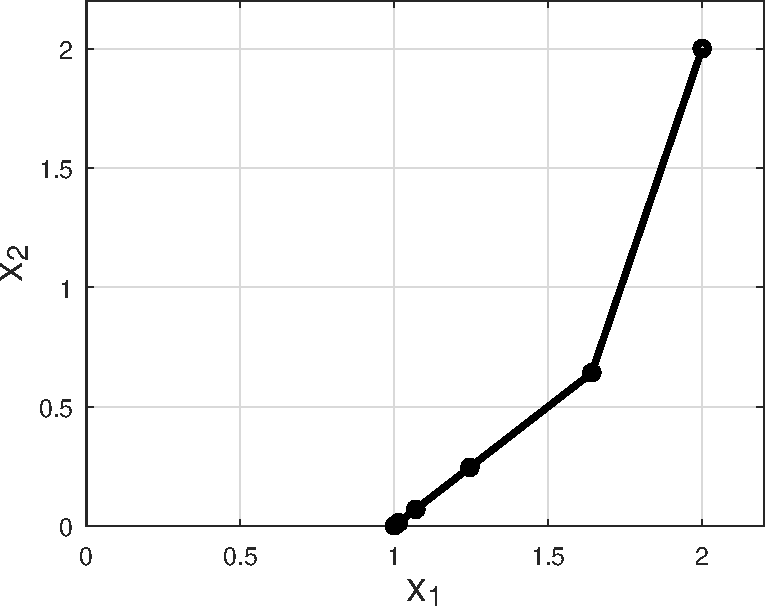
\includegraphics[width=0.45\textwidth]{figs/small.pdf} \qquad 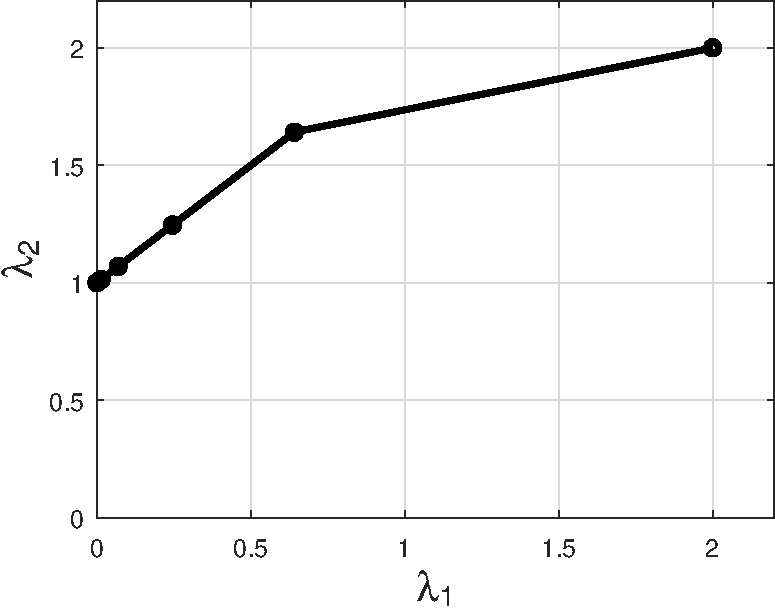
\includegraphics[width=0.46\textwidth]{figs/smalldual.pdf}}


\subsubsection*{Example 2.}

The next problem is an $n=5$ linear programming (LP) problem, in standard form, with $m=3$ linear equality constraints:
\begin{equation}
\begin{matrix}
\text{minimize} \qquad & f(x) = c^\top x \\
\text{subject to} \qquad & A x = b \\
 & x \ge 0
\end{matrix} \label{eq:linearproblem}
\end{equation}
where $\ds c = \begin{bmatrix} -1 & -2 & 0 & 0 & 0 \end{bmatrix}^\top$, $\ds A = \begin{bmatrix} -2 & 1 & 1 & 0 & 0 \\ -1 & 2 & 0 & 1 & 0 \\ 1 & 0 & 0 & 0 & 1 \end{bmatrix}$, and $\ds b = \begin{bmatrix} 2 & 7 & 3 \end{bmatrix}^\top$.

\begin{wrapfigure}[12]{r}{0.35\textwidth}
\phantom{x} \hfill 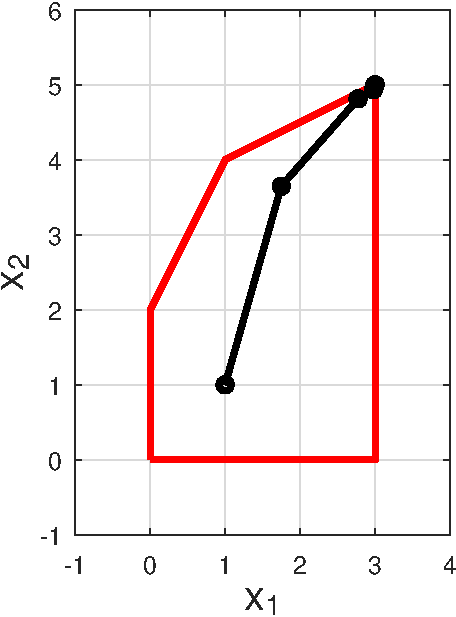
\includegraphics[width=0.3\textwidth]{figs/linear.pdf}
\end{wrapfigure}

\medskip
This problem is solved by the simplex method in \cite[section 5.2]{GrivaNashSofer2009}.  Starting from $x=0$ the simplex method finds the solution on the third iteration.

Standard-form problem \eqref{eq:linearproblem} arises from 2D LP problem
\begin{equation}
\begin{matrix}
\text{minimize} \qquad & z = -x_1 - 2x_2 \\
\text{subject to} \qquad & -2x_1 + x_2 \le 2 \\
 & -x_1 + 2x_2 \le 7 \\
 & x_1 \le 3 \\
 & x_1, x_2 \ge 0
\end{matrix} \label{eq:twodlp}
\end{equation}
This feasible set of \eqref{eq:twodlp} can be easily sketched (at right).

Problem \eqref{eq:linearproblem} is defined in a short driver program \href{https://github.com/bueler/popdip/blob/main/matlab/linear.m}{\texttt{linear.m}}.  It runs POPDIP with initial iterate $x_0=(1,1,1,1,1)^\top$ and \texttt{rtol} $=10^{-14}$, otherwise using the default parameters.  The result is strongly superlinear convergence similar to Example 1:
\begin{Verbatim}[fontsize=\footnotesize]
>> linear
        x_1                  x_2                  nu_k                 mu_k
  0:    1.000000000000000    1.000000000000000    5.477225575051662
  1:    1.749124060578910    3.650175187884218    2.662463982283214    0.547722557505166
  2:    2.771966360502739    4.813544496010846    0.673064121890067    0.266246398228321
  3:    2.977196636050274    4.937189711618397    0.151356274478520    0.067306412189007
  4:    2.993139910878286    4.988863175677374    0.033061726195566    0.015135627447852
  5:    2.999412769621014    4.999167116475287    0.002445966295331    0.001093077739031
  6:    2.999996717485349    4.999995406776724    0.000013394027090    0.000005982751118
  7:    2.999999999901378    4.999999999862158    0.000000000401658    0.000000000179400
  8:    3.000000000000000    5.000000000000000    0.000000000000000    0.000000000000000
\end{Verbatim}

The 2D iterates $x_k$ are shown in the figure.  This would appear to be good performance of an interior-point method on an LP problem.  Compare figure 5.1, chapter 10, and section 10.6 in \cite{GrivaNashSofer2009}.

It is worth considering the Newton step equations \eqref{eq:newtonstep} in this LP case.  Because the objective function $f(x) = c^\top x$ is linear, the gradient $\grad f=c$ is constant and the Hessian is zero, so \eqref{eq:newtonstep} becomes
\begin{equation}
\begin{bmatrix}
X_k^{-1}\Lambda_k  & -A^\top \\
-A                 & 0
\end{bmatrix}
\begin{bmatrix}
\Delta x \\
\Delta \tau
\end{bmatrix}
=
\begin{bmatrix}
-c + A^\top \tau_k + \mu_k X_k^{-1} e \\
A x_k - b
\end{bmatrix}. \label{eq:lpnewtonstep}
\end{equation}
The square system matrix on the left of \eqref{eq:lpnewtonstep} is invertible when $\mu_k>0$.  (This is proven in the Appendix.  One only needs the facts that $A$ has full row rank and that $\mu_k\ne 0$.)  Thus it is okay, as shown by this example, to supply a zero Hessian.

Regarding application of POPDIP to LP problems, one might ask how it does on the famously-bad Klee-Minty cube example \cite[chapter 9]{GrivaNashSofer2009}.  The answer for now is ``not any better than simplex''!   Presumably the parameters and details could be adjusted to improve the performance.\footnote{See the discussion of following the central path in chapter 14 of \cite{NocedalWright2006}.}  In any case we can compare the results of the \href{https://github.com/bueler/popdip/blob/main/matlab/kmpopdip.m}{\texttt{kmpopdip.m}} example code here to the result of

\medskip
\centerline{\href{https://bueler.github.io/opt/assets/codes/F24/simplex/kleeminty.m}{\texttt{bueler.github.io/opt/assets/codes/F24/simplex/kleeminty.m}}}

\medskip
\noindent which uses the simplex method.  Both seem to generate exponentially-increasing numbers of iterations as the dimension of the cube increases.


\subsubsection*{Example 3.}

Next we consider a continuum (infinite-dimensional) optimization problem with positivity constraints.  The discretized problem has arbitrary size $n$, but otherwise the problem is like Example 1; it is a quadratic optimization with only nonnegativity constraints.

The continuum problem is an \emph{obstacle problem} \cite[chapter 12]{Bueler2021},
\begin{equation}
\begin{matrix}
\text{minimize} \qquad & f(u) \\
\text{subject to} \qquad & u \ge 0
\end{matrix} \label{eq:obstacleproblem}
\end{equation}
where
\begin{equation}
    f(u) = \int_0^1 \frac{1}{2} u'(x)^2 - q(x) u(x)\,dx. \label{eq:obstaclefcn}
\end{equation}
The admissible functions $u(x)$ in \eqref{eq:obstacleproblem} must be continuous and have one well-defined (i.e.~$L^2$) derivative on the interval $0\le x \le 1$.  Furthermore we assume boundary conditions $u(0)=u(1)=0$.

If $y=u(x)$ gives the height of a taught string which is pinned at the ends then we may interpret $\frac{1}{2} u'(x)^2$ in \eqref{eq:obstaclefcn} as its elastic energy.  This quantity becomes larger as there are more bends in the graph of $u(x)$.  In this context the continuous source function $q(x)$ is an external upward/downward force on the string.  The reason \eqref{eq:obstacleproblem} is called an ``obstacle'' problem \cite{KinderlehrerStampacchia1980} is that the zero function, the obstacle in this case, stops the solution from going further down even if negative values of $q(x)$ would force it down: $u(x)\ge 0$.

Source functions $q(x)$ which are both negative and positive are of primary interest because they generate a free boundary at a point $x=\alpha$ where $u(\alpha)=0$ and $u'(\alpha)=0$, although $u(x)$ is positive on one side of $\alpha$.  (See the derivation of the exact solution \eqref{eq:obstacleexactsolution} below for a particular case.)  However, when $q(x)\le 0$ everywhere then one may show that $u(x)\equiv 0$ is the global minimizer.  On the other hand, if $q(x)\ge 0$ everywhere and $q(x) > 0$ at any one point then $u(x)>0$ on the whole open interval $(0,1)$, so the inequality constraint is nowhere active.

The discretization replaces $u(x)$ by a continuous and piecewise-linear function, so we are applying a finite element method\footnote{It can also be interpreted as finite differences \cite{LeVeque2007}.} \cite{Elmanetal2014}.  These functions are linear between the points of a pre-determined grid on $[0,1]$.  Let $x_i$ be points $x_0 = 0 < x_1 < x_2 < \dots < x_n < x_{n+1}=1$, here equally-spaced for simplicity.  Then $\Delta x = 1 / (n+1)$ is the spacing and we have $x_i = i\Delta x$.  Only the interior grid points are locations of (primal) variables in the optimization problem \eqref{eq:obstacleproblem}: $u = (u_1,\dots,u_n)^\top \in \RR^n$ where $u_i=u(x_i)$.

Now we approximate the objective function \eqref{eq:obstaclefcn} using the midpoint numerical integration rule.  In the interval $(x_i,x_{i+1})$ the slope of $u(x)$ is $(u_{i+1}-u_i)/\Delta x$, and the midpoint value of $u(x)$ is $u(x_{i+1/2}) = (u_i + u_{i+1})/2$.  Also we assume $q(x)$ is given by a formula which we may evaluate at will.  The discrete objective function is, therefore,
\begin{equation}
    f_n(u) = \frac{\Delta x}{2} \sum_{i=0}^n \left(\left(\frac{u_{i+1}-u_i}{\Delta x}\right)^2 - q(x_{i+1/2}) (u_i + u_{i+1})\right) \label{eq:discobstaclefcn}
\end{equation}
where the endpoint values are $u_0=0$ and $u_{n+1}=0$ when they appear.  (These are notational conveniences and not actual variables.)  Observe that \eqref{eq:discobstaclefcn} is actually a whole class of example objective functions, for different functions $q(x)$.  For each dimension $n=1,2,3,\dots$ there is a finite-dimensional optimization problem derived from the continuum problem \eqref{eq:obstacleproblem}.

It follows that the gradient is
\begin{equation}
\left(\grad f_n(u)\right)_i = \frac{1}{\Delta x} \left\{\begin{matrix}
2 u_1 - u_2 & (i=1) \\
-u_{i-1} + 2 u_i - u_{i+1} & (1<i<n) \\
-u_{n-1} + 2 u_n & (i=n) \\
\end{matrix} \right\} - \frac{\Delta x}{2} (q(x_{i-1/2}) + q(x_{i+1/2}))
\end{equation}
for $i=1,\dots,n$.  Since the objective function is quadratic, its Hessian is a constant matrix, of a form well-known to be positive-definite \cite{LeVeque2007}:
\begin{equation}
\grad^2 f_n(u) = \frac{1}{\Delta x} \begin{bmatrix}
2  & -1 &    &    \\
-1 &  2 & -1 &    \\
   &    & \ddots &\\
   &    & -1 &  2
\end{bmatrix}
\end{equation}

\newcommand{\uex}{u_{\text{exact}}}
To test the accuracy of the implementation we must find an exact solution $\uex(x)$ to the continuum problem.  This solution will not be an exact solution to any of the discrete problems, so for finite $n$ we will not know the exact minimizer $u_* \in \RR^n$ of $f_n(u)$.  However, because our discretization is convergent \cite{Elmanetal2014,LeVeque2007}, for large $n$ the finite-dimensional minimizer $u_*$ should be close to the grid values $\uex(x_i)$.  If we solve the $f_n(u)$ optimization problem accurately then our numerical minimizer $u\in\RR^n$ should be close to $u_*\in\RR^n$, and thus also close to $\uex(x)$.  In any case, we will measure the total numerical error, the norm of the grid point errors $|u_i - \uex(x_i)|$.

The continuum exact solution $\uex(x)$ solves \eqref{eq:obstacleproblem} for $q(x) = -100 (\cos(2\pi x) + 0.7)$; this source function is shown in the left plot below.  The details of this $q(x)$ are not special except that $q(x)$ is positive on a small interval around $x=0.5$, specifically on $(0.3734,0.6266)$.  The exact solution $\uex(x)$ is found by observing that the (strong form) NCP form of problem \eqref{eq:obstacleproblem} is
\begin{equation}
u(x) \ge 0, \qquad - u''(x) - q(x) \ge 0, \qquad u(x) (- u''(x) - q(x)) = 0.  \label{eq:obstaclencp}
\end{equation}
The solution to \eqref{eq:obstacleproblem} and \eqref{eq:obstaclencp} is symmetric around $x=0.5$ because $q(x)$ is symmetric around that point.  A free boundary \cite{KinderlehrerStampacchia1980} will arise at a location $0<\alpha<0.5$ where $u(\alpha)=0$ and $u'(\alpha)=0$.  Combining these facts gives the formula\footnote{This is a nonobvious calculation.  In summary, one starts from $u''=-q$, and integrates once, setting the constant using symmetry $u'(0.5)=0$.  Then use $u'(\alpha)=0$ to determine $\alpha$ by solving a transcendental equation: $\sin(2\pi \alpha)/(2 \pi) + 0.7 (\alpha - 0.5)=0$.  (I used Newton's method to compute $\alpha$ to 15 digits.)  Then integrate again to find $u(x)$, and use $u(\alpha)=0$ to set the constant.  The result is \eqref{eq:obstacleexactsolution}.}
\begin{equation}
\uex(x) = \begin{cases} 0, & 0 \le x \le \alpha \\
                        100 \left(\frac{\cos(2\pi\alpha) - \cos(2\pi x)}{(2\pi)^2} - \frac{0.7}{2} (\alpha (\alpha-1) - x (x-1))\right), & \alpha < x < 1-\alpha \\
                        0, & 1-\alpha \le x \le 1. \end{cases}  \label{eq:obstacleexactsolution}
\end{equation}
Here $\alpha=0.275562026630539$ gives the exact (i.e.~very accurate) location $x=\alpha$ of the free boundary on the interval $0<x<0.5$.  By symmetry there is a matching free boundary on $0.5<x<1$, namely at $1-\alpha$.

\medskip
\noindent \mbox{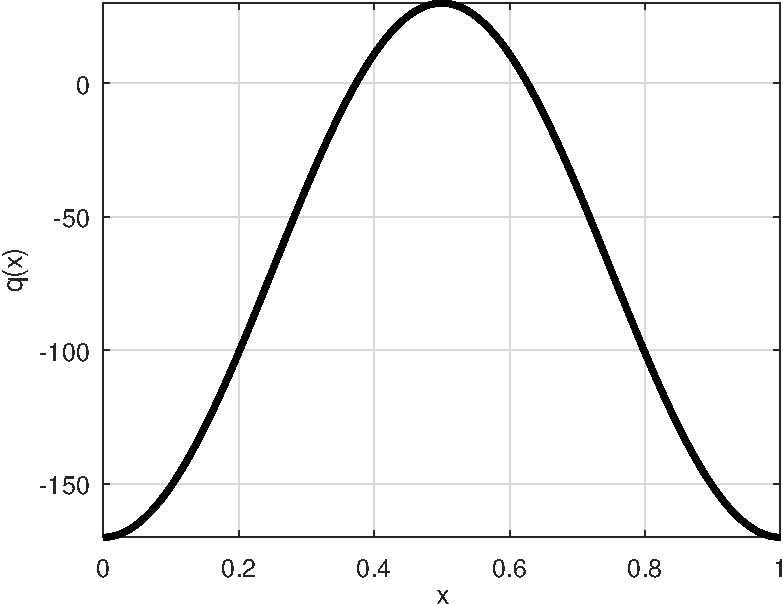
\includegraphics[width=0.47\textwidth]{figs/qobstacle.pdf} \qquad
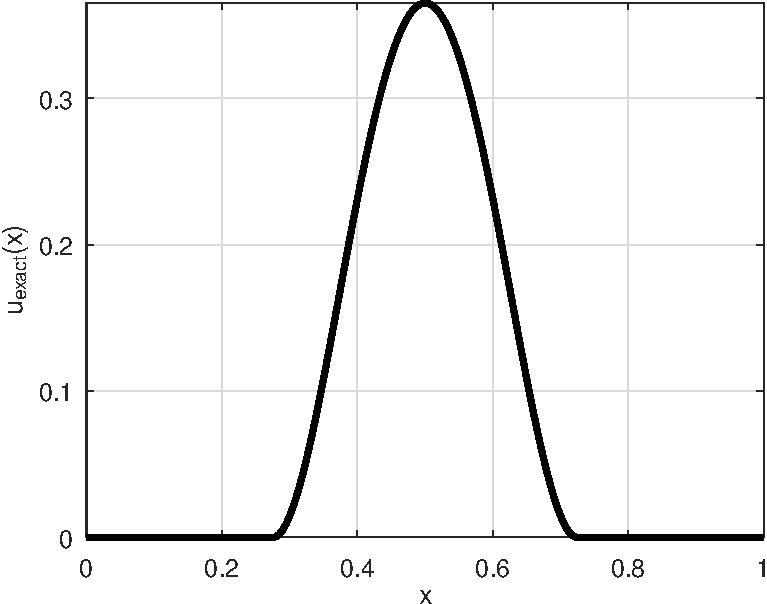
\includegraphics[width=0.47\textwidth]{figs/uexactobstacle.pdf}}

The exact solution is plotted in the right figure.  Note that the set on which $\uex(x)= 0$, i.e.~where the constraint is active, is a strict subset of the set on which $q(x)<0$, where there is a downward force on the string.  Finding the free boundary $x=\alpha$, where the string first meets the obstacle, is a typical goal for this kind of problem.

Formula \eqref{eq:obstacleexactsolution} appears in the short driver program \href{https://github.com/bueler/popdip/blob/main/matlab/obstacle.m}{\texttt{obstacle.m}}.  Because the exact solution is known, the numerical error can be measured at the end.  The program calls POPDIP with initial iterate $(u_0)_i=1$, and parameters \texttt{rtol} $=10^{-12}$ and \texttt{theta} $=0.001$, otherwise using the defaults.  The user-supplied objective function $f_n(u)$, namely \eqref{eq:obstaclefcn}, and the gradient, Hessian, and the formula for $q(x)$, all appear in the function \href{https://github.com/bueler/popdip/blob/main/matlab/obstaclefcn.m}{\texttt{obstaclefcn.m}}, the handle of which is also passed to POPDIP.

By default \href{https://github.com/bueler/popdip/blob/main/matlab/obstacle.m}{\texttt{obstacle.m}} uses $n=25$ interior grid points.  The output merit function $\nu_k$ values, and the dynamically-adjusted barrier parameters $\mu_k$, suggest strongly superlinear convergence similar to previous Examples:
\begin{Verbatim}[fontsize=\footnotesize]
>> obstacle
        nu_k                 mu_k
  0:   42.668104033897947
  1:    5.652366439731654    0.042668104033898
  2:    1.582225195585537    0.005652366439732
  3:    0.405205172171047    0.001582225195586
  4:    0.244137215303266    0.000405205172171
  5:    0.201522593604293    0.000244137215303
  6:    0.107490917285153    0.000201522593604
  7:    0.029115141695205    0.000107490917285
  8:    0.000205231703144    0.000029115141695
  9:    0.000017959316470    0.000000042120052
 10:    0.000000001669991    0.000000000322537
 11:    0.000000000000004    0.000000000000000
12 iterations with n=25: ||u-uexact||_inf = 6.557e-03
\end{Verbatim}

The final numerical error norm $\|u-\uex\|_\infty = 6.557 \times 10^{-3}$ shows that $u\in\RR^{25}$ is close to the continuum exact solution at the grid points.  On the other hand, our tolerance \texttt{rtol} $=10^{-12}$ has made $u$ \emph{much} closer to the constrained optimum $u_*$ of $f_{25}(u)$.  That is, most of the numerical error is discretization error, which we can only reduce by choosing larger $n$.\footnote{Or by choosing a different discretization scheme.  One might want to use a spectral method, but it will not work easily for obstacle problems!}

The run also produces the figures below.  The initial iterate $u_0=1$ (left figure) is far from the correct solution.  We see above that the merit function value $\nu_k$ stagnates for a while before starting superlinear convergence.  The right figure shows both the primal $u(x)$ and the dual $\lambda(x)$ numerical solutions, for which complementarity ($u_i \lambda_i=0$) is clear.  Note that the numerical error $|u_i-\uex(x_i)|$ jumps up from zero abruptly at the free boundary.\footnote{In fact $\uex(x)$ has a discontinuous second derivative at the free boundary $x=\alpha$.  There is no way for a piecewise-linear function to do a good job of approximating it.}

\medskip
\noindent \mbox{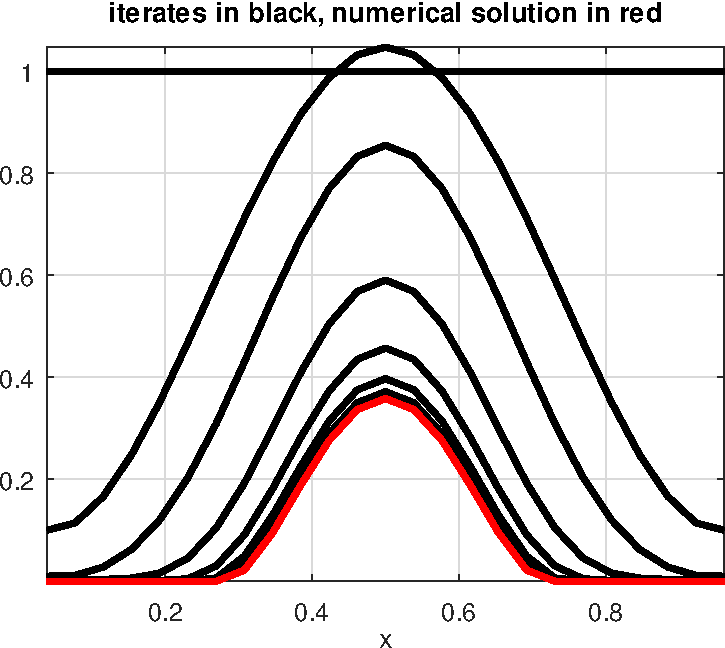
\includegraphics[width=0.45\textwidth]{figs/iteratesobstacle.pdf} \qquad
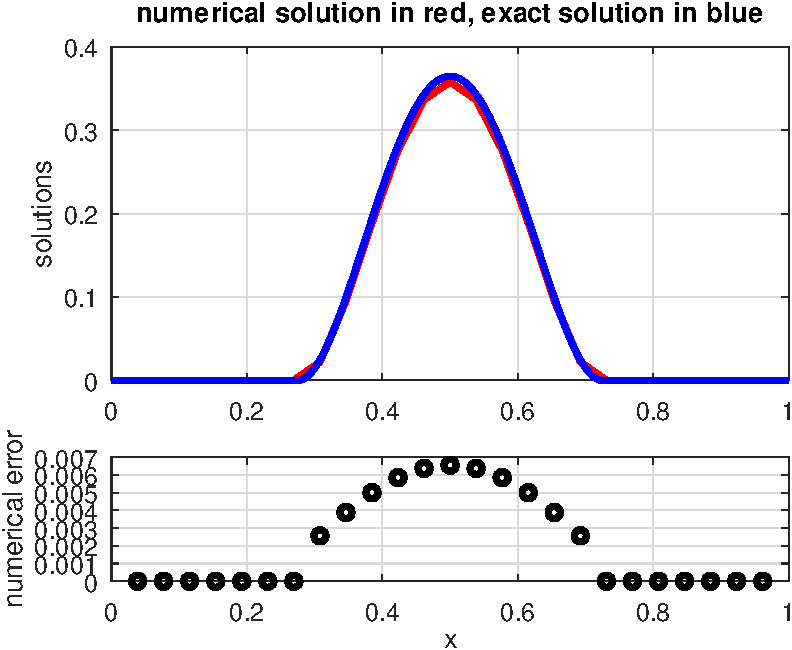
\includegraphics[width=0.5\textwidth]{figs/errorobstacle.pdf}}

The reader might experiment with larger $n$ values.  The numerical error is an order of magnitude smaller after two grid-doubling refinements to $n=100$.  The POPDIP algorithm is not so well-behaved under further refinement; significantly smaller numerical error is hard to achieve.  (The reasons are not all clear to me.)


%\subsubsection*{Example 4.}
%FIXME Application to glacier problem.  Note a primal-dual interior point method for a glacier problem appears in \cite{Calvoetal2003}


\subsection*{Possible improvements}

POPDIP is an implemented primal-dual interior point method, but it is far from the best algorithm which experts could create.  The following is a non-exhaustive list of possible improvements.

\begin{itemize}
\item The step sizes $\alpha$ can be chosen more carefully so that the iterates $x_k,\tau_k,\lambda_k$ remain in a neighborhood of the central path.  Chapter 14 of \cite{NocedalWright2006} may be a good reference, but see also \cite{YamashitaYabe1996} and \cite{ZhangTapiaDennis1992}.  Section 14.2 of \cite{NocedalWright2006} describes a predictor-corrector scheme which might be more efficient.
\item For nonquadratic objective functions $f(x)$ one should add a line search, presumably a sufficient-decrease line search as in \cite[section 11.5]{GrivaNashSofer2009} and \cite[sections 19.3, 19.4]{NocedalWright2006}.  See also the modified back-tracking line searches in \cite{BensonMunson2006}.
\item For nonconvex objective functions $f(x)$ we could adjust the Hessian block in system \eqref{eq:newtonstep} to always be positive definite so that the unconstrained primal step would be a descent direction.  See \cite[section 11.4]{GrivaNashSofer2009}.
\item We could apply scalable linear algebra, presumably preconditioned Krylov methods \cite{Bueler2021}, so that when matrices are sparse, as in Example 3, the solution of system \eqref{eq:newtonstep} is faster.
\item One could apply the quasi-Newton idea to construct an approximation of the Hessian block in system \eqref{eq:newtonstep}, so that the user does not need to supply a Hessian.  See sections 12.3 and 13.5 of \cite{GrivaNashSofer2009} and section 19.3 of \cite{NocedalWright2006}.
\end{itemize}


\medskip

\bibliography{doc}
\bibliographystyle{siam}

\appendix
\subsection*{Appendix: Invertibility of the system matrix}

\newtheorem*{lemma}{Lemma}
\newtheorem*{corollary}{Corollary}

Recall from \eqref{eq:equalities} that if $\mu_k>0$ then $x_k,\lambda_k$ are strictly positive.  It follows that the diagonal matrices $\Lambda_k,X_k$ in \eqref{eq:unreducednewtonstep} are invertible.

\begin{lemma}
Suppose $\grad^2 f(x_k)$ is positive semi-definite.  Then the $(n+m)\times (n+m)$ symmetric matrix in linear system \eqref{eq:newtonstep} is invertible.
\end{lemma}

\begin{proof}  Let $K=\grad^2 f(x_k)+X_k^{-1}\Lambda_k$.  It is easy to see that $K$ is positive definite, thus invertible, since $X_k^{-1}\Lambda_k$ is diagonal with positive diagonal entries.

Suppose the system matrix has a null space:
\begin{equation}
\begin{bmatrix}
K   & -A^\top \\
-A  & 0
\end{bmatrix}
\begin{bmatrix}
\Delta x \\
\Delta \tau
\end{bmatrix}
= 0. \label{eq:invertlp}
\end{equation}
The first row of \eqref{eq:invertlp} says
    $$K \Delta x = A^\top \Delta\tau,$$
equivalently $\Delta x = K^{-1} A^\top \Delta \tau$.  Now the second row of \eqref{eq:invertlp}, $A\Delta x=0$, can be written as an equation for $\Delta\tau$:
    $$A K^{-1} A^\top \Delta \tau = 0.$$
Since $K^{-1}$ is also positive definite, it has a Cholesky decomposition \cite{TrefethenBau1997}, so $K^{-1}=LL^\top$ where $L$ is $n\times n$, lower triangular, and invertible.  Recall that since $A$ has full row rank its columns span $\RR^m$, thus $AL$ also has full row rank.  But then $A K^{-1} A^\top = (AL) (AL)^\top$ is positive definite, thus invertible, so $\Delta \tau=0$.  Now $\Delta x=0$, so the null space is trivial.  It follows that the matrix is invertible. \end{proof}

\begin{corollary} The system matrix in LP problem \eqref{eq:lpnewtonstep} is invertible.
\end{corollary}

\begin{proof}  The zero matrix is positive semi-definite.  \end{proof}

Note that in \eqref{eq:lpnewtonstep} we have $K^{-1}=\Lambda_k^{-1} X_k=D^2$, with positive diagonal factors $D$, as the Cholesky decomposition.  The quirky article by Strang \cite{Strang1987} expands on the importance of matrices $A D^2 A^\top$ where $D$ is an invertible diagonal matrix and $A$ has full row rank.

\end{document}

